\documentclass[a4paper,11pt]{article}
\usepackage[T1]{fontenc}
\usepackage{inputenc}
\usepackage{amsfonts}
\usepackage{graphicx}
\usepackage{bm}
\usepackage{varioref}
\usepackage[english]{babel}
\usepackage{hyperref}
\usepackage{tikz}
\usepackage[vmargin=3.5cm]{geometry}
\newcommand{\field} [1] {\mathbb{#1}}
\begin{document}

\begin{titlepage}
\centering \parindent=0pt
\newcommand{\HRule}{\rule{\textwidth}{1mm}}
\vspace*{\stretch{1}} \HRule\\[1cm]\Huge\bfseries
Roadmap\\[0.7cm]
\large The visualisation\\[1cm]
\HRule\\[4cm]  \large by \\Jacob Stenum Czepluch (jstc@itu.dk), \\Niels Liljedahl Christensen (nlch@itu.dk), \\Mikkel Larsen (milar@itu.dk), \\Sigurt Bladt Dinesen (sidi@itu.dk) \\
\vspace*{\stretch{2}} \normalsize %
\begin{flushleft}
IT-University\\
Copenhagen\\
First year project\\
Rasmus Pagh\\
\today \end{flushleft}
\end{titlepage}

\tableofcontents
\pagebreak

\pagebreak
\section{Introduction}

This report covers the visualisation part of our first-year project at the MSc in Software Development at the IT-University of Copenhagen. This first part has been made in March and April in the year 2012. 

To make this project, we were randomly divided into groups of size four to six. Our group, group 8, consists of four students. 

The main purpose of this project is to visualise road-map data provided by Krak. The data is to be visualised as a map displaying all roads within a given square area of Denmark.
It must be possible to zoom in and out on a desired part of the map. In addition, the level of detail should should follow the zoom level. It is also required that the window in which the map is displayed can be resized. In the description of our assignment, a few  optional, possible additions to the program were suggested. 

There are worksheets corresponding to the work we have made at, and due to every meeting. The worksheets also contain information about agreements formed in the introductory phase of the project, as well as agreements formed throughout the project.

Our advisor throughout this project has been Rasmus Pagh, from whom we have received both guidence and relevant lectures. 

Furthermore we would like to thank Robert Sedgewick and Kevin Wayne from Princeton University for providing well written and easy-to-understand code and algorithms at \url{algs4.cs.princeton.edu} that we have chosen to use and rewrite for our data structure in this project.

\pagebreak
\section{Design choices} % (fold)
\label{sec:Design choices}
In this section, we will go through our design choices. We will go through things like design patterns, data structures, and visualisation.
At the same time we will explanation our choices.

\subsection{Design Pattern} % (fold)
\label{sub:Design Pattern}
For our overall architectural pattern, we have chosen to use the Model, View, Controller (MVC) pattern. We chose to do so, to make sure that we have
a very modular and easy-to-maintain class structure. Using the MVC pattern results in seperation of the different aspects of our application, while still providing a loose coupling between these elements. During this first visualisation part of the application it has proven very useful to us since we
have been chancing our classes and data structures quite a few times.

% subsection Design Pattern (end)

\subsection{Data Structure} % (fold)
\label{sub:Data Structure}
We started out by making a simple data structure that put all the edges into one big \texttt{ArrayList}. This was not fast, but we chose to do it, to make sure that
things were working before we tried implementing a more complicated, but faster, data structure. We have had several data structures up for discussion, but we ended up using a quadtree. We actually started out making a k-D tree, but since we had some trouble implementing it correctly, we decided to take a look at
the quadtree as well. Luckily it turned out to perform very well, and we did not even have to sort our input for it to work well. In our discussion 
section we will further elaborate on the pros and cons of the different data structures.
% subsection Data Structure (end)

\subsection{Visualisation} % (fold)
\label{sub:Visualisation}

% subsection Visualisation (end)

\subsubsection{Platform} % (fold)
\label{subsub:Platform}
To start with we had to decide whether we wanted to use \texttt{Java} and \texttt{Swing}, or \texttt{Java}, \texttt{JavaScript}, \texttt{SVG}, and \texttt{HTML} for the visualisation part. There are strengths and weaknesses to both solutions: The good thing about \texttt{Swing} is that we all have previous experience with it, and so we were certain that, using \texttt{Swing}, we would be able to do what we wanted. 
The fact that none of us have had any notable experience with \texttt{JavaScript} and \texttt{SVG} made it easy for us to decide on a platform for this project. By using \texttt{Java} and \texttt{Swing}, we would be able to spend our time making a well working program with a nice data structure. We would, of course, have liked looking into a new language like \texttt{JavaScript}, but we have chosen to prioritize a well working program over the learning experience of working with a new programming language.
% subsubsection Platform (end)

\subsubsection{How everything is drawn} % (fold)
\label{subsub:How everything is drawn}
As mentioned above we chose to use \texttt{Swing} and the \texttt{BasicStroke API} to do the drawing of the map. 

Technically, the map first draws all of Denmark. It is however only the two biggest road types that are drawn in the full view. We decided to only do so because it is both unnecessary to draw all roads when you are very far away from the map, but also to make the program run smoother. The program is designed to show more and more road types the more you zoom in towards the map. Only the roads that are inside the given view are drawn. We have, however, made a "buffer" that finds the longest road in the view, and extends the frame outside the view with the given length. This is done to make sure that all roads in the view are drawn and visible.
% subsubsection How everything is drawn (end)

\subsubsection{User interaction} % (fold)
\label{subsub:User interaction}
We wanted to make a simple, yet featureful, user interface. This resulted in a user interface with no physical buttons. All you need to navigate the map is pointing device (i.e., a mouse). To zoom in and out you scroll up and down, respectively. The mouse pointer decides what the zooming point is. It is also very easy to pan up or down, or to the sides. This is done by simply dragging and dropping the map with the mouse pointer. The window is also easily resized by dragging in one corner of the window. There are, however, some differences in the way that the resizing behaves according to the OS the program is running under.

Our main reason for designing the user interface the way that we have is that, in our strongest conviction, it is the most intuitive way for people to navigate and interact with maps. It seems that this has become the \textit{de facto} standard, probably due to the increasing number of tablets and smartphones on the market.
% subsubsection User interaction (end)

\pagebreak
\section{Implementation} % (fold)
\label{sec:Implementation} % This sections should describe our implementation
The implementation of the application consists of four different packages; the \texttt{Model}, \texttt{View} and \texttt{Controller} packages used as in the MVC design pattern, and a \texttt{Global} package storing global fields to be accessed and modified from all other packages.


\subsection{Controller package} % This is a simple description of the implementation of the Controller class.
The \texttt{Controller} package consists solely of the \texttt{Controller} class, which is both the main class (it has the main method, to be run when the application starts), and it is the link between the \texttt{Model} and \texttt{View} packages handling the flow of data between the two. When a change is made by the user, the \texttt{View} calls a method in the \texttt{Controller}, once again updating the graphical user interface according to user input and the data stored in the \texttt{Model}.

\subsection{Global package} % Contains all the global values used from all around the application
This package contains only the \texttt{MinAndMaxValues} class which has fields that need to be accessed from the entire application. These fields include initial values such as the current "viewbox", minimum and maximum values for x- and y-coordinates, definitions for when the different types of road segments are drawn etc. It also contains methods for checking whether or not the current viewbox results in a need for re-filtering the data to be drawn. The class is statically imported by all classes needing to access this information.

\subsection{Model package} % The description of the Model package is more complicated and consists of descriptions of several other classes.
%The \texttt{Model} package consists of all the classes managing data storage, filtering, and conversion.

\subsubsection{Model class} % Makes use of the rest of the classes in the Model package. The front-end class.
The \texttt{Model} class is the front-end class of the \texttt{Model} package (the only class which is directly connected to the \texttt{Controller} class). This is where the data structure is stored in a field and where the methods for filtering and converting data are called. The data structure is stored with the type \texttt{DataStructure}, which is an interface allowing us to easily switch between data structures.

\subsubsection{XMLReader class} % Reads in the data from an XML file of krax format and adds the content to a given data structure
This class reads data from an XML file of our KRAX format and converts it to instances of the \texttt{Edge} class (a simple class representing an edge on the roadmap), which are then added to a given data structure.

The \texttt{XMLReader} makes use of an external library, \href{www.xom.nu}{\texttt{xom}} (\url{www.xom.nu}), for reading the XML data.

\subsubsection{QuadTreeDS class} % The data structure of the application. Consists of several other classes to be explained here
The \texttt{QuadTreeDS} is the basis of the entire application. It is in an instance of this class that all data is stored after being read by the \texttt{XMLReader} class. In order for it to be used as our data structure, it implements the \texttt{DataStructure} interface.

The class consists of four instances of the \texttt{QuadTree} class (one for each type of road segment). A \texttt{QuadTree} consists of nodes, which has an x- and a y-coordinate (stored as \texttt{double}s) and a reference to an \texttt{Edge} object. Each \texttt{QuadTree} contains all edges of a designated type. Each \texttt{Edge} object is stored twice; both referenced to by the start- and end-coordinates of the edge.

Inserting a node into a \texttt{QuadTree} is a recursive process; the given node is compared to the root node, deciding which of the four children the given node is to be compared with next. This continues until a null-reference / a leaf is found.

Retrieving information is done using an instance of the \texttt{Interval2D} class (representing a rectangle), which again consists of two instances of the \texttt{Interval} class (each representing a line). This too is done recursively; it is checked whether the coordinates of the root node are within the given rectangle. If it is, it is added to a given collection of edges. It is then checked which of the subtrees might contain nodes within the rectangle, and for each that match, the same method is invoked, now with each of the matching children as the root. The call returns at null references.

Our implementation of the quadtree (including the \texttt{Interval} and \texttt{Interval2D} classes) is heavily based upon implementations from \url{algs4.cs.princeton.edu}.
\\
\begin{figure}[!h]
\centering
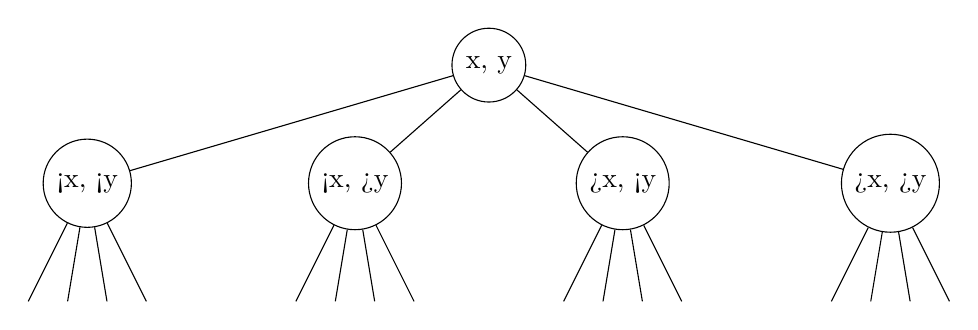
\begin{tikzpicture}
	[level 1/.style={sibling distance=34mm},
	level 2/.style={sibling distance = 5mm}]
	\tikzstyle{every node}=[circle,draw]
	\node {x, y}		
		child {
			node {<x, <y}
			child
			child
			child
			child
		}
		child {
			node {<x, >y}
			child
			child
			child
			child		
		}
		child {
			node {>x, <y}
			child
			child
			child
			child		
		}
		child {
			node {>x, >y}
			child
			child
			child
			child		
		}
	;
\end{tikzpicture}
\end{figure}
\\
\subsubsection{FormatConverter class} % Converts from the data type pulled out of the data structure to the data type needed by the View package
The \texttt{FormatConverter} has static methods only, and only one public method. This methods takes an \texttt{ArrayList<Edge>} and converts it to the type \texttt{int[][][]} \\(\texttt{int[type][number of edges][edge coordinates]}).

The FormatConverter uses an instance of the Coordinates class to convert the given UTM32 coordinates to pixels as shown in the GUI.

\subsubsection{KrakToXMLConverter class} % Not directly part of the implementation, but the class used for converting the data from Krak to the krax XML format
The KrakToXMLConverter is not, strictly speaking, a part of the application (it is not used at runtime). It is a utility class, reading in the data supplied by Krak, writing it to an XML file of the KRAX format (once again using the external \href{www.xom.nu}{\texttt{xom}} library).

\subsection{View package} % Consists of all the classes handling the graphical user interface
%The \texttt{View} package contains all the classes managing the graphical user interface.

\subsubsection{View class} % Front end class in the MVC pattern. Contains the rest of the (non-static) GUI classes. Implements the MapListener interface. The overall class structure of the View package
The \texttt{View} class is the front-end class of the \texttt{View} package in the MVC design pattern. It contains an instance of the \texttt{MainFrame} class, which is the basic \texttt{java.swing} GUI (the window to be displayed), which then again contains an instance of our custom panel, \texttt{MapPanel}.

The \texttt{View} itself implements the interface \texttt{ViewListener}, of which an instance is stored in both the \texttt{MainFrame} and the \texttt{MapPanel} classes. This allows for these classes to invoke a method in the \texttt{View}, telling it that changes has been made, which then invokes a similar method in the \texttt{Controller}, which then updates the GUI according the the changes.

\subsubsection{MapPanel class} % Draws lines according to input data
The \texttt{MapPanel} class extends the \texttt{java.swing.JPanel} class and functions as a panel with extended functionality and with an overridden \texttt{paint} method.

The \texttt{MapPanel} stores an \texttt{int[][][]} (as generated by the \texttt{FormatConverter}), from which it draws lines of the canvas, each corresponding to an edge stored in the \texttt{Model}.

The \texttt{MapPanel} also has two listeners from the \texttt{java.awt} library; a \\\texttt{MouseWheelListener}, which invokes a static method of the \texttt{ZoomHandler} class when the user scrolls on the panel, sending data about the mouse coordinates and the scrolled amount, and a \texttt{MouseMotionListener}, which invokes a static method of the \texttt{DragHandler} class when the user drags the mouse on the panel, letting the \texttt{DragHandler} know how far the mouse has been dragged (and along which axes).

\subsubsection{ZoomHandler class} % Handles all the zooming
The \texttt{ZoomHandler} handles all zooming. When a call is received (from the \texttt{MapPanel}), signaling that the user wishes to zoom out, there are two possible outcomes: If the current viewbox is not too close to the maximum width and height values; it zooms out, maintaining the current center of the viewbox. Otherwise, if the viewbox is near its extrema, zooming is done with the viewbox bound to the borders imposed by the maximum values.

Subsequently to zooming in, a call is made to the \texttt{DragHandler} class, moving the viewbox towards the current location of the cursor.

Zooming is simply a matter of changing the global values indicating what is being displayed (in the \texttt{MinAndMaxValues} class) / changing the size of the viewbox and then invoking a repaint of the \texttt{MapPanel}.

\subsubsection{DragHandler class} % Handles all the dragging
The \texttt{DragHandler} class, like the \texttt{ZoomHandler} class, changes the viewbox according to input data (drag amount and direction) and according the the maximum values that definine the extrema of the viewbox.

\pagebreak
\section{Discussion} % (fold)
\label{sec:Discussion} % In this sections we will discuss what could have been done better, and/or what we think we have done right
Several decisions, affecting both application performance and user interaction, have been made during the implementation. The most relevant ones will be discussed here.

\subsection{Platform} % The discussion of zooming and window resizing on different platforms
Currently, the application has been tested on computers running Mac OS X and Arch Linux, and some differences concerning the application exists.

When resizing the window on Mac OS X, no message is sent to the application until the user stops resizing (releases the mouse button). On Arch Linux, each time the window is resized the slightest, a message is sent. We have therefore decided not to keep a constant width-height ratio, since this does not work correctly on a computer running Arch Linux, though this would be our preferred design choice. Instead, only the content of the frame is changed, in accordance to the the resizing being done.

When zooming on Mac OS X, a message with a number is sent, representing an amount to be zoomed. On Arch Linux however, the size of the number is always 1, making the zooming a very slow process.

\subsection{Data structure} % Includes the discussion of QuadTree vs KD-tree and Balanced vs unbalanced QuadTree. And one QuadTree vs 4 QuadTrees

\subsubsection{Quadtree or k-D tree} % The discussion of quadtree vs KD-tree
We have decided on a quadtree for our data structure. We believe that we could have got a similar result using k-D trees. The k-D trees have the advantage that they are easy to balance. Quadtrees have the advantage that they have an overall smaller height, due to the nature of the k-D trees being binary trees.

\subsubsection{Balanced or unbalanced quadtree} % The discussion of whether or not the quadtree should be balanced
We have made experiments balancing our quadtrees, choosing pivot elements in different ways and partitioning the rest of the data, doing this recursively. However, the improvements we experienced were very slight, which is why our current implementation uses unbalanced quadtrees.

\subsubsection{Our use of four quadtrees} % The discussion of whether or not it is a good idea that we use several quadtrees as our data structure
Our current data structure consists of four quadtrees, one per type of edge stored. This means the application has to search through several quadtrees, if several types are to be drawn. It would be preferable having everything in the same tree, allowing the overall tree height (the sum of all our tree heights) to be smaller. But since we only have four quadtrees, we believe that the performance difference would be un-noticeable.

\subsection{Inclusion of optional assignments} % How we gave a proper data structure and a proper basis higher priority than many features
We have decided to give the implementation of our data structure and and the basic user interaction with the application higher priority than including extra, optional features.
% section Discussion (end)

\pagebreak
\section{Conclusion} % (fold)
\label{sec:Conclusion}
To conclude and sum up this first part of the project, we are very happy with the way our project has turned out so far. 

Our group has a good dynamic way of working and we are good at keeping deadlines and meeting times. This has made it easy for us to focus on making
capable design choices and making our program work as intended. And we have succeeded in making a program that works as intended. One could argue that our program could be a bit quicker, but we are convinced that our program is fast enough for its purpose, and we have not experienced any mentionable slowdowns. 

There are few things would have wanted to do differently, if we were to re-do this project. We would have liked to add more of the optional features to the program, as we have only included one; a fast data structure.
It is possible to navigate the application using touchpad only, and the implementation of the overall navigation works as intended in the design.
Our final project will in all likelines have more extraneous features and improvements added to the application.

We are, all in all, very pleased with both our work as a group, and our program so far.
%Our group has had a very good and dynamic teamwork. We have been good at keeping deadlines and meeting times, which has lead to a product that we are very satisfied with.
% section Conclusion (end)

\end{document}
